\documentclass[main.tex]{subfiles}
\begin{document}
\section{Results}
Sample executions of the simulation outlined in section \ref{sec:simulation} have been
performed. As a starting point a lab side length of \(1\) mm was chosen, the lattice
granularity was set to \(101^3\) sites and the current running through each coil was
selected as \(10\) A. All graphs presented are drawn with metres as axis units. In light of the typical Stern-Gerlach experiment the total mass
of the dumbbell was initially assumed to be \(3.58\times 10^{-25}\) kg, the mass of two silver
atoms, and additionally the distance between the two dumbbell masses was set to \(5\times
10^{-5}\) m. At first a distance on the order of Ångström was trialled, but nonzero
spin-spin coupling \(J\) then led to rotational accelerations too large for the ODE solver
to handle. The velocity by which the dumbbell enters the lab was \(1\) cm/s in the positive
\(x\) direction for all simulations. A maximum simulation time of \(0.1\) s was
assumed, but this matters only for the high energy state
since the other
trajectories exit the lab before then. The graphs shown have been ''swarmed'', by which it
is here meant that several simulations of equal parameters have been placed at equidistant
initial positions along the \(yz\) plane. Note also further that the linearity of the
external magnetic field strength \(B\) with respect to the current \(I\) means that any multiplication of that
variable will yield the same effect as an equal change in the spin-field coupling
\(\gamma\), since the field strength and coupling parameter always appear as a single product. For this reason the current of the magnetic field will in general be held fixed
and \(\gamma\) will be varied instead, as this does not require additional field
generation.

The scripts print average force magnitudes for the different terms in equation
\ref{eq:dynfin}. For brevity's sake these are not displayed in full here, but will be
quoted when appropriate. Note also that the rotation of the dumbbell, while simulated and
while it does affect the centre off mass trajectory, is not plotted.

First all three possible eigenstates were tested for the given parameters, and with
\(\gamma = 10^{10}\) J/(\(\hbar{}\)T), \(J = 10^5\) J/\(\hbar{}\), see figure
\ref{fig:ncompare}. For all of these simulations the gradient of the fast Hamiltonian
energy was the dominating term by a factor \(\sim 10^{5}\), but note the large differences
in behaviour of this non-synthetic action. This is the expected behaviour, as discussed in
section \ref{sec:nonsynbeh}
, but note for now that the low energy state is repelled away from the lab and is thus not
very useful. The high energy state is ''caught'' between the coils while the middle state
achieves but a perturbed straight motion through the lab.
\begin{figure}[h]
    \centering
    \subfloat[\centering \(n =
    0\)]{{\includegraphics[width=4cm]{figures/n_compare/I10nr101lablength0.001tmax0.1J100000.0Gamma10000000000.0mass3.58e-25len5e-05n0vel(0.01,
            0, 0, 0, 0)swarmnum4norotFalsenosynFalse}}}
    \qquad
    \subfloat[\centering \(n = 1\)]{{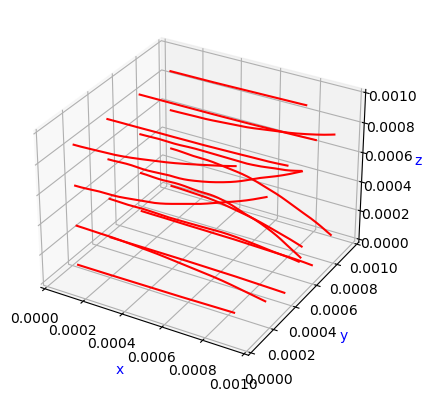
\includegraphics[width=4cm]{figures/n_compare/I10nr101lablength0.001tmax0.1J100000.0Gamma10000000000.0mass3.58e-25len5e-05n1vel(0.01, 0, 0, 0, 0)swarmnum4norotFalsenosynFalse}}}
    \qquad
    \subfloat[\centering \(n = 2\)]{{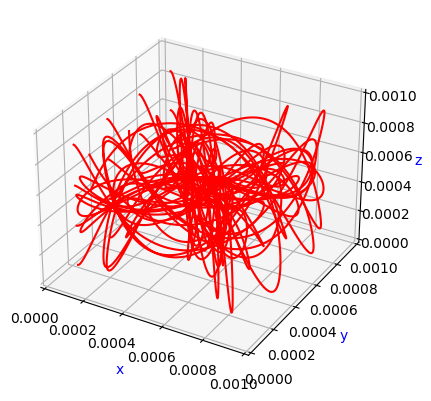
\includegraphics[width=4cm]{figures/n_compare/I10nr101lablength0.001tmax0.1J100000.0Gamma10000000000.0mass3.58e-25len5e-05n2vel(0.01, 0, 0, 0, 0)swarmnum4norotFalsenosynFalse}}}
    \caption{\centering All three eigenstates simulated for \(\gamma = 10^{10}\) J/\(\hbar{}\), \(J = 10^5\)
    J/\(\hbar{}\).}%
    \label{fig:ncompare}
\end{figure}
Motion for the same parameters but excluding synthetic field effects were simulated, see
figure \ref{fig:ncompare_nosyn}. Note that the nonsynthetic dynamics dominate completely.
While small differences can be found they are miniscule, and may very well lie within the
error of the simulation.
\begin{figure}[h]
    \centering
    \subfloat[\centering \(n =
    0\)]{{\includegraphics[width=4cm]{figures/n_compare_nosyn/I10nr101lablength0.001tmax0.1J100000.0Gamma10000000000.0mass3.58e-25len5e-05n0vel(0.01,
            0, 0, 0, 0)swarmnum4norotFalsenosynTrue}}}
    \qquad
    \subfloat[\centering \(n =
    1\)]{{\includegraphics[width=4cm]{figures/n_compare_nosyn/I10nr101lablength0.001tmax0.1J100000.0Gamma10000000000.0mass3.58e-25len5e-05n1vel(0.01,
    0, 0, 0, 0)swarmnum4norotFalsenosynTrue}}}
    \qquad
    \subfloat[\centering \(n =
    2\)]{{\includegraphics[width=4cm]{figures/n_compare_nosyn/I10nr101lablength0.001tmax0.1J100000.0Gamma10000000000.0mass3.58e-25len5e-05n2vel(0.01,
    0, 0, 0, 0)swarmnum4norotFalsenosynTrue}}}
    \caption{All three eigenstates simulated for \(\gamma = 10^{10}\) J/\(\hbar{}\), \(J = 10^5\)
    J/\(\hbar{}\), without synthetic field effects.}%
    \label{fig:ncompare_nosyn}
\end{figure}
\subsection{The middle state}\label{sec:resmiddle}
Let now attention be turned to the \(n = 1 \) case. If the nonsynthetic term is to be
reduced in size, such that the synthetic field effects become visible, a reduction in fast
Hamiltonian energy is desired. Note that for the special case \(J = 0\) the fast
Hamiltonian diagonalizes, and the middle state will simply have the energy zero. This
change in parameter yields a graph such as the one to the left in figure \ref{fig:noJ1}. As predicted the fast
energy is now identically zero, up to a numerical error of order \(\sim 10^{-44}\) J, and since that was previously the dominating term motion is
simply rectilinear. While hardly a usable result in it self, it is now notable that the
synthetic contributions to the dynamics are generally many orders of magnitude larger than the
fast energy gradient, which is but a numerical residue on the order of \(\sim 10^{-37}\) N.
The magnitude of the synthetic forces, on the order of \(\sim 10^{-31}\) N for the magnetic
field
and \(\sim 10^{-33}\) N for the scalar field, are simply too small in comparison to the
dumbbell mass.
\begin{figure}[h]
    \centering
    \subfloat[\centering \(J =
    0\), \(n = 1\), \(m = 3.58\times 10^{-25}\) kg]{{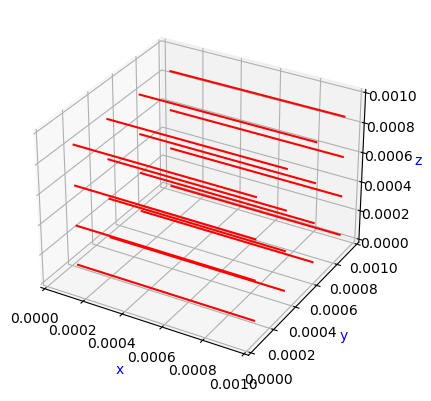
\includegraphics[width=4cm]{figures/J0/I10nr101lablength0.001tmax0.1J0Gamma10000000000.0mass3.58e-25len5e-05n1vel(0.01, 0, 0, 0, 0)swarmnum4norotFalsenosynFalse}}}
    \qquad
    \subfloat[\centering \(J = 0\), \(n =
    1\), \(m = 3.58\times 10^{-28}\) kg]{{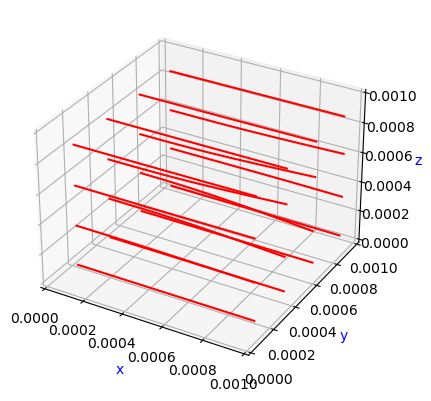
\includegraphics[width=4cm]{figures/J0/I10nr101lablength0.001tmax0.1J0Gamma10000000000.0mass3.58e-28len5e-05n1vel(0.01, 0, 0, 0, 0)swarmnum4norotFalsenosynFalse}}}
    \qquad
    \subfloat[\centering \(J = 0\), \(n =
    1\), \(m = 3.58\times 10^{-29}\) kg]{{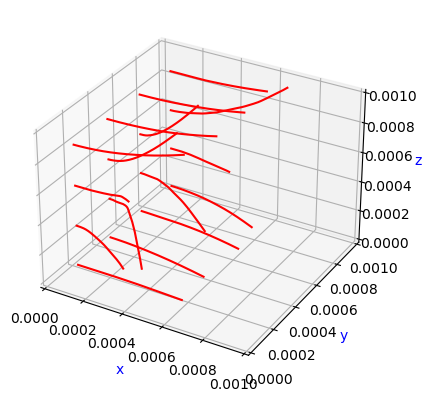
\includegraphics[width=4cm]{figures/J0/I10nr101lablength0.001tmax0.1J0Gamma10000000000.0mass3.58e-29len5e-05n1vel(0.01, 0, 0, 0, 0)swarmnum4norotFalsenosynFalse}}}
    \caption{\centering Three different masses for \(n = 1\), \(J = 0\)}%
    \label{fig:noJ1}
\end{figure}

Any simple tool for increasing the action of the synthetic fields is however absent. As can
be noted both by parallell to the geometric phase and directly from equations \ref{eq:FA}
and \ref{eq:ElPot} the synthetic potentials are generally not dependent on the magnitude of
the fast energy. As of such direct increases of parameters \(J\) and \(\gamma\) will typically
have the effect of increased nonsynthetic action while the synthetic fields are not
strengthened. Also relevant is the dependence of the synthetic magnetic field on the
velocity of the dumbbell. However, much like the motion through a classical magnetic field
the impulse from a Lorentz-type force over a fixed distance is independent on the velocity,
as the travel time scales reciprocally to the force magnitude. The lab length could be
adjusted, but here too would the effects on the synthetic magnetic field action cancel out.
Imagine that the velocity were kept constant in relation to the lab side length.
Multiplying the side length by any factor would then scale the velocity equally. However
the derivatives present in equation \ref{eq:FA} would scale reciprocally, and nothing would
be achieved.

All that is left is then to adjust the mass of the dumbbell, as this affects nothing but
the resultant acceleration. Reduction of mass yields perceptible effects first
at the order of \(\sim 10^{-28}\) kg, and at \(\sim 10^{-29}\) kg, as visible in figure
\ref{fig:noJ1}. %Unrealistic masses
The dumbbell is clearly repelled from the point of energy degeneration, as is the predicted
behaviour of the synthetic scalar field per section \ref{sec:BOinterp}. That this behaviour
is due to the synthetic fields only is clear from simulations run without synthetic
dynamics, see figure \ref{fig:noJ2}. That the scalar synthetic field now dominates even
though the numbers cited earlier for the ''high'' mass case would indicate otherwise can be
traced to that the printed force magnitudes are averaged out over the trajectory, so a
difference in trajectory will affect the average force values. Specifically if the scalar
field repels the dumbbell away from the lab a larger proportion of the trajectory will be
close to the centre and thus the average scalar force will increase. This is visible in the
printouts, for the rightmost case in figure \ref{fig:noJ1} the average synthetic scalar
force is of order \(\sim 10^{-30}\) N.

\begin{figure}[h]
    \centering
    \subfloat[\centering \(J =
    0\), \(n = 1\), \(m = 3.58\times 10^{-25}\)
    kg]{{\includegraphics[width=4cm]{figures/J0/I10nr101lablength0.001tmax0.1J0Gamma10000000000.0mass3.58e-25len5e-05n1vel(0.01,
    0, 0, 0, 0)swarmnum4norotFalsenosynTrue}}}
    \qquad
    \subfloat[\centering \(J = 0\), \(n =
    1\), \(m = 3.58\times 10^{-28}\)
    kg]{{\includegraphics[width=4cm]{figures/J0/I10nr101lablength0.001tmax0.1J0Gamma10000000000.0mass3.58e-28len5e-05n1vel(0.01,
    0, 0, 0, 0)swarmnum4norotFalsenosynTrue}}}
    \qquad
    \subfloat[\centering \(J = 0\), \(n =
    1\), \(m = 3.58\times 10^{-29}\)
    kg]{{\includegraphics[width=4cm]{figures/J0/I10nr101lablength0.001tmax0.1J0Gamma10000000000.0mass3.58e-29len5e-05n1vel(0.01,
    0, 0, 0, 0)swarmnum4norotFalsenosynTrue}}}
    \caption{\centering Three different masses for \(n = 1\), \(J = 0\), without synthetic field
    effects.}%
    \label{fig:noJ2}
\end{figure}

That it is indeed the synthetic scalar field repelling the trajectories from the
centre point can be confirmed through running simulations without either the synthetic
scalar or magnetic field, as has been done in figure \ref{fig:noJ3}

\begin{figure}[h]
    \centering
    \subfloat[\centering \(J =
    0\), \(n = 1\), \(m = 3.58\times 10^{-29}\)
    kg, no synthetic scalar field]{{\includegraphics[width=4cm]{figures/J0/I10nr101lablength0.001tmax0.1J0Gamma10000000000.0mass3.58e-29len5e-05n1vel(0.01,
    0, 0, 0, 0)swarmnum4norotFalsenosynNoscalar}}}
    \qquad
    \subfloat[\centering \(J = 0\), \(n =
    1\), \(m = 3.58\times 10^{-29}\)
    kg, no synthetic magnetic field]{{\includegraphics[width=4cm]{figures/J0/I10nr101lablength0.001tmax0.1J0Gamma10000000000.0mass3.58e-29len5e-05n1vel(0.01,
    0, 0, 0, 0)swarmnum4norotFalsenosynNomag}}}
    \caption{\centering The final simulation of figure \ref{fig:noJ1} without the synthetic scalar or
    magnetic fields}%
    \label{fig:noJ3}
\end{figure}
Note that the impact of the synthetic magnetic field as in the leftmost graph is not
completely negligible, but does constitute a visible perturbation to the rectilinear
motion. Further reduction of the mass to increase the synthetic magnetic dynamic lead
however to no interesting patterns.

It should be noted that such large reductions of mass as have been done makes the
results rather unstable to numerical errors. It can be noted in many graphs above that the
trajectories are not fully symmetric as one would expect in the perfect case, but that
numerical perturbations propagate. It would be a stretch to call the behaviour 'chaotic',
but the exact trajectories should not be taken for more than examples of qualitative
behaviour.

The more exotic synthetic field given by a nonzero value of \(J\) would be of interest to
consider, but regrettably leads to a sharp increase in the fast eigenvalues. This puts a
limit to the size of the parameter which can be simulated before the dumbbell is quickly
expelled from the lab, but sample simulations of \(J = 100\) J/\(\hbar{}\) were performed
in figure \ref{fig:n1Je2}. Note here the dependence on whether synthetic field effects are
included. Once again it is the synthetic scalar effects that dominate.
\begin{figure}[h]
    \centering
    \subfloat[\centering \(J =
    0\), \(n = 1\), \(m = 3.58\times 10^{-29}\)
    kg, no synthetic scalar
    field]{{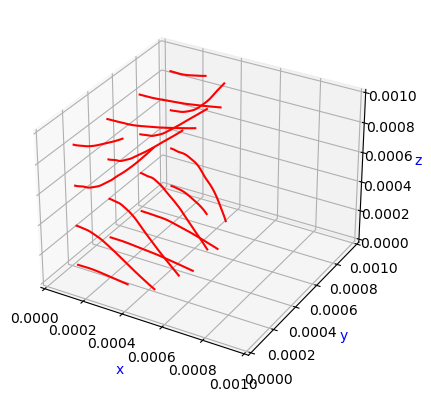
\includegraphics[width=4cm]{figures/n1Je2/I10nr101lablength0.001tmax0.1J100.0Gamma10000000000.0mass3.58e-29len5e-05n1vel(0.01, 0, 0, 0, 0)swarmnum4norotFalsenosynFalse}}}
    \qquad
    \subfloat[\centering \(J = 0\), \(n =
    1\), \(m = 3.58\times 10^{-29}\)
    kg, no synthetic magnetic
    field]{{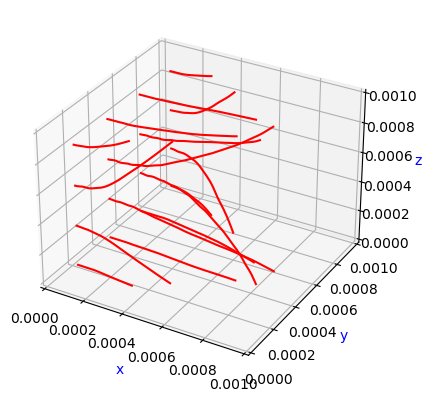
\includegraphics[width=4cm]{figures/n1Je2/I10nr101lablength0.001tmax0.1J100.0Gamma10000000000.0mass3.58e-29len5e-05n1vel(0.01, 0, 0, 0, 0)swarmnum4norotFalsenosynTrue}}}
    \caption{\centering Simulations for the middle state with nonzero \(J\), both with synthetic field
    effects and without.}%
    \label{fig:n1Je2}
\end{figure}


\subsection{The high energy state}\label{sec:reshigh}
The behaviour of the nonsynthetic fields to ''trap'' the dumbbell between the coils if
placed in the high energy state is promising. Even if the fast energy gradient can be
assumed to dominate the behaviour, the prospect of the synthetic fields acting on the
dumbbell for extended periods of time suggests perhaps notable perturbations to the
nonsynthetic motion. As seen in figure \ref{fig:ncompare} the graphs are quickly cluttered
when several starting positions are considered at once, and so a different ''swarming''
procedure was adopted. Choosing a single starting position and velocity trajectories owing
to different choices of fields contributing were performed simultaneously, and subsequently
coloured thereafter for visibility. Furthermore the simulation time was increased to half a
second as to propagate the synthetic perturbations as much as possible without obstructing
visibility too much.

This then infers a choice of starting position. Several such choices were sampled, here are
presented the most interesting ones found as of yet. Further reducing the number of
starting positions and parameters possible is the fact that some trajectories cross the
degeneration at the centre, prohibiting field action comparison. Such choices of parameters
are not shown here. 

\begin{figure}[h]
    \centering
    \subfloat[\centering With synthetic fields in red,
    without in blue]{{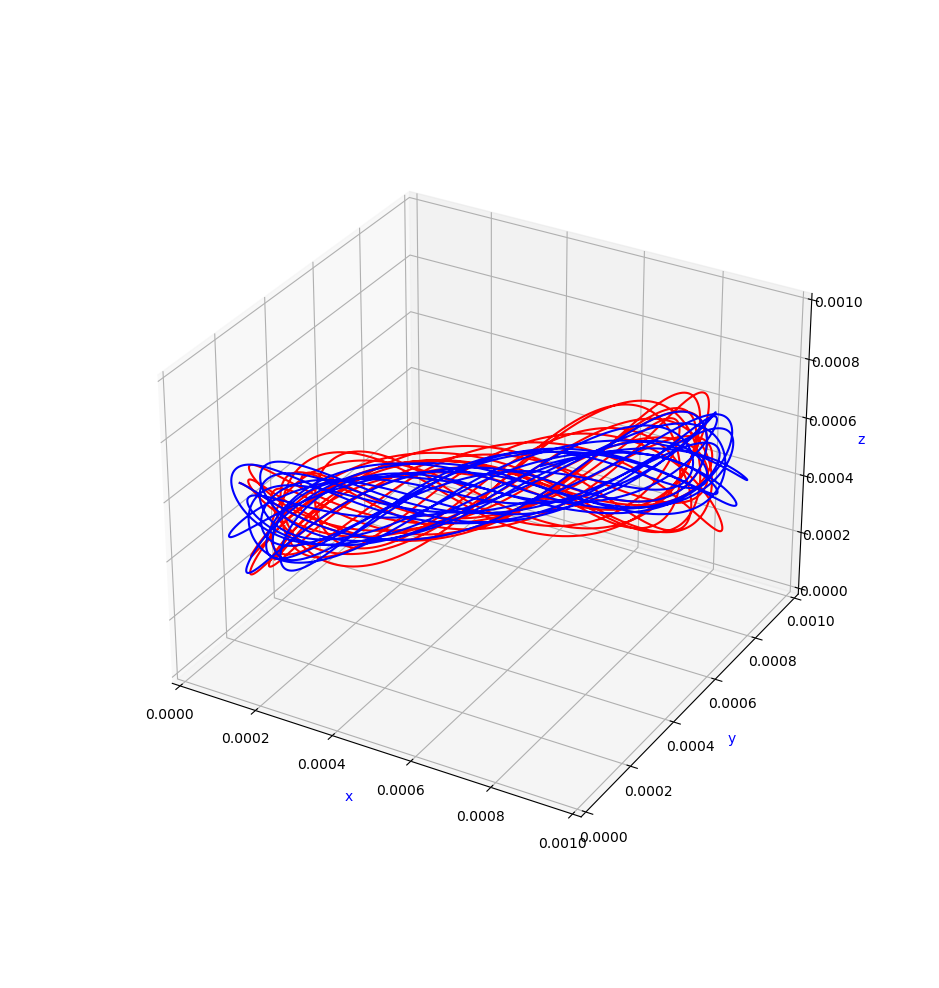
\includegraphics[width=7cm]{figures/n2m-25/(0,2)-comp1}}}
    \qquad
    \subfloat[\centering Without synthetic magnetic field in green,
    without synthetic scalar field in yellow]{{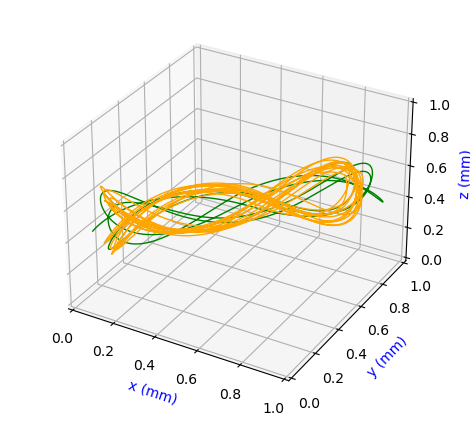
\includegraphics[width=7cm]{figures/n2m-25/(0,2)-comp2}}}
    \caption{\centering Simulations of the high energy state at a fixed starting position for \(\gamma
    = 10^{10}\) J/\(\hbar{}\), \(J= 10^{5}\) H/\(\hbar{}\).}%
    \label{fig:n2m-25}
\end{figure}

First simulations of the same parameters as in figure \ref{fig:ncompare} were performed for
a starting position close to \(y=0\) mm and \(z = \frac{3}{4}\) mm, see figure
\ref{fig:n2m-25}. Note the clearly visible perturbation of the synthetic field on the trajectory,
and note further the large influence of the synthetic magnetic field on the trajectory
compared to the synthetic scalar field. Direct comparison between the trajectory without
synthetic fields at all and the trajectory without the synthetic magnetic field show large
similarities, but still perturbation by the synthetic field is noticeable. It can be
concluded that the synthetic magnetic field plays a major role in repelling the trajectory
from the slim cylinder traversed otherwise as seen in the left hand side of figure \ref{fig:n2m-25}. This is also
supported by the average force values, which for the present simulation were of the order
\(\sim 10^{-29}\) N for the synthetic magnetic field, \(\sim 10^{-34}\) N for the synthetic
scalar field and \(\sim 10^{-24}\) N for the fast energy gradient.

\begin{figure}[h]
    \centering
    \subfloat[\centering With synthetic fields in red,
    without in blue]{{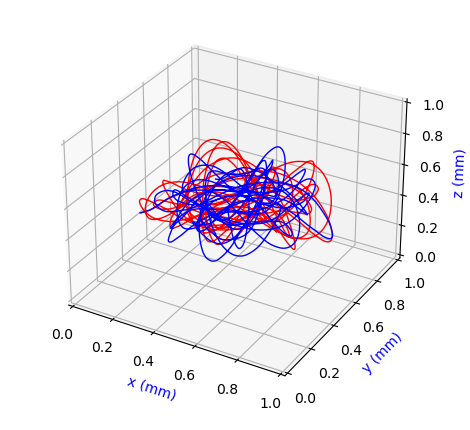
\includegraphics[width=7cm]{figures/n2m-27/(1,1)-comp1}}}
    \qquad
    \subfloat[\centering Without synthetic magnetic field in green,
    without synthetic scalar field in yellow]{{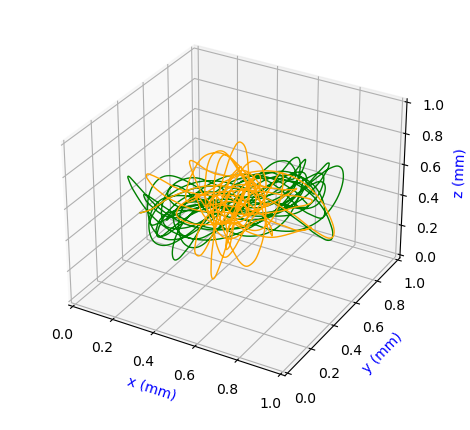
\includegraphics[width=7cm]{figures/n2m-27/(1,1)-comp2}}}
    \caption{\centering Simulations of the high energy state at a fixed starting position for \(\gamma
    = 10^{8}\) J/\(\hbar{}\), \(J= 10^{5}\) H/\(\hbar{}\), \(m = 3.58\times 10^{-27}\) kg.}%
    \label{fig:n2m-27A}
\end{figure}

Just like the discussion in section \ref{sec:resmiddle} concluded reduction of mass is the
main tool for increase of synthetic magnetic field effects. To this end simulations were
run for a mass of \(3.58\times 10^{-27}\) kg, where the spin-field coupling constant was
adjusted accordingly to \(\gamma = 10^{8}\) J/\(\hbar{}\) such that the fast energy
acceleration remained approximately the same, see figure \ref{fig:n2m-27A}. The starting
position was close to \(y= \frac{1}{4}\) mm and \(z = \frac{1}{4}\) mm. Here the
synthetic effects can easily be said to play a significant role in the
dynamics of the system. Qualitative descriptions of the behaviour are not from the onset
very clear however, except that the synthetic scalar field appears to somewhat confine the
motion, or in the very least reduce the rotation about the system \(z\)-axis. That all
contributions to the dynamics play noticeable roles can be seen from the pairwise
comparisons of figure \ref{fig:n2m-27B}. For these simulations the magnitude of the
synthetic scalar and magnetic forces were of the same order of \(\sim 10^{-28}\) N, while
the fast energy gradient was of the order \(10^{-26}\) N.
%Hanteln roterar även nu ordentligt, och slutade upp på theta aprx. 4 och phi aprx. 100

\begin{figure}[h]
    \centering
    \subfloat[\centering With synthetic fields in red,
    without synthetic magnetic field in green]{{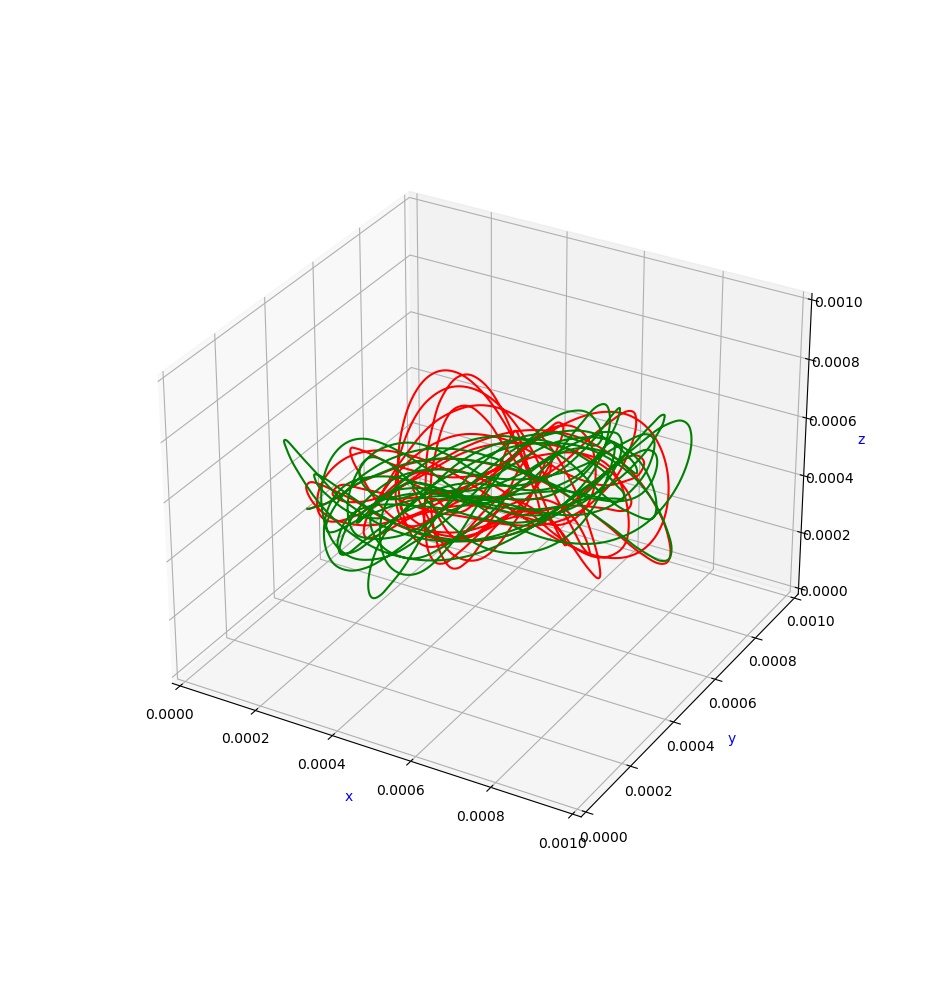
\includegraphics[width=7cm]{figures/n2m-27/(1,1)-comp3}}}
    \qquad
    \subfloat[\centering With synthetic fields in red,
    without synthetic scalar field in yellow]{{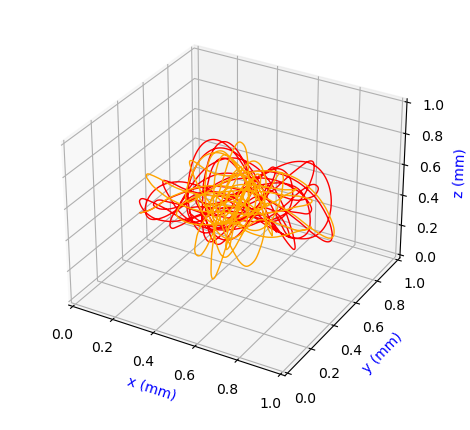
\includegraphics[width=7cm]{figures/n2m-27/(1,1)-comp4}}}
    \qquad
    \subfloat[\centering Without synthetic magnetic field in
    green, without both synthetic fields in blue]{{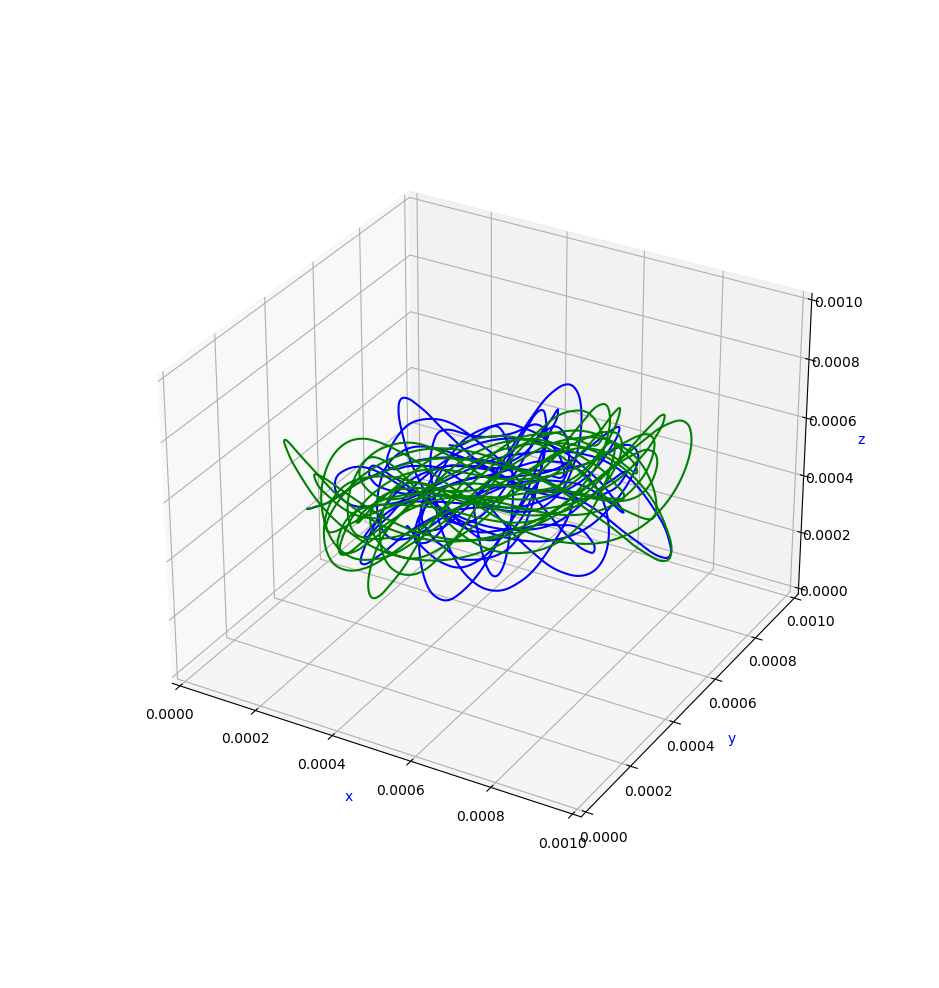
\includegraphics[width=7cm]{figures/n2m-27/(1,1)-comp5}}}
    \qquad
    \subfloat[\centering Without synthetic scalar field in
    yellow, without both synthetic fields in blue]{{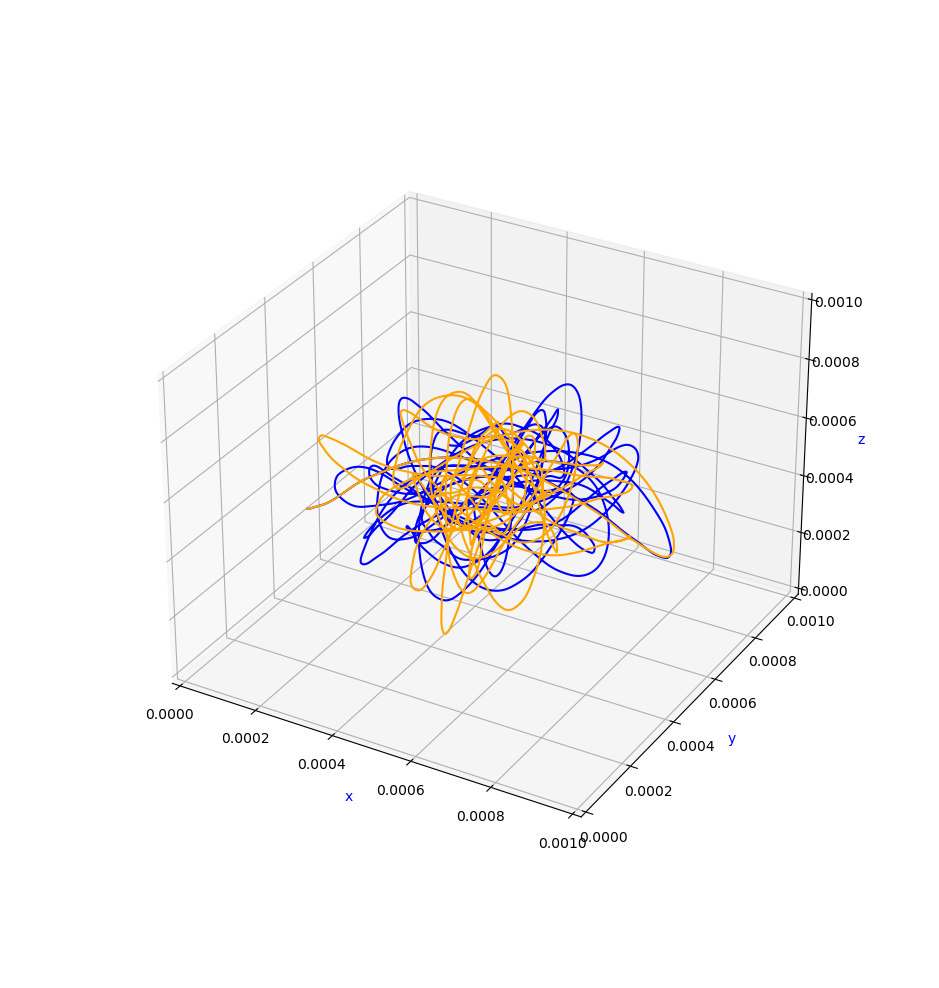
\includegraphics[width=7cm]{figures/n2m-27/(1,1)-comp6}}}
    \caption{\centering Simulations of the high energy state at a fixed starting position for \(\gamma
    = 10^{8}\) J/\(\hbar{}\), \(J= 10^{5}\) H/\(\hbar{}\), \(m = 3.58\times 10^{-27}\) kg.}%
    \label{fig:n2m-27B}
\end{figure}
\end{document}
